\section{Realisering og test}
\label{sec:research}

Kretsen ble realisert i programmet Icestudio som vist i figur \ref{fig:ICE}

\begin{figure}[!hbt]
	\centering
	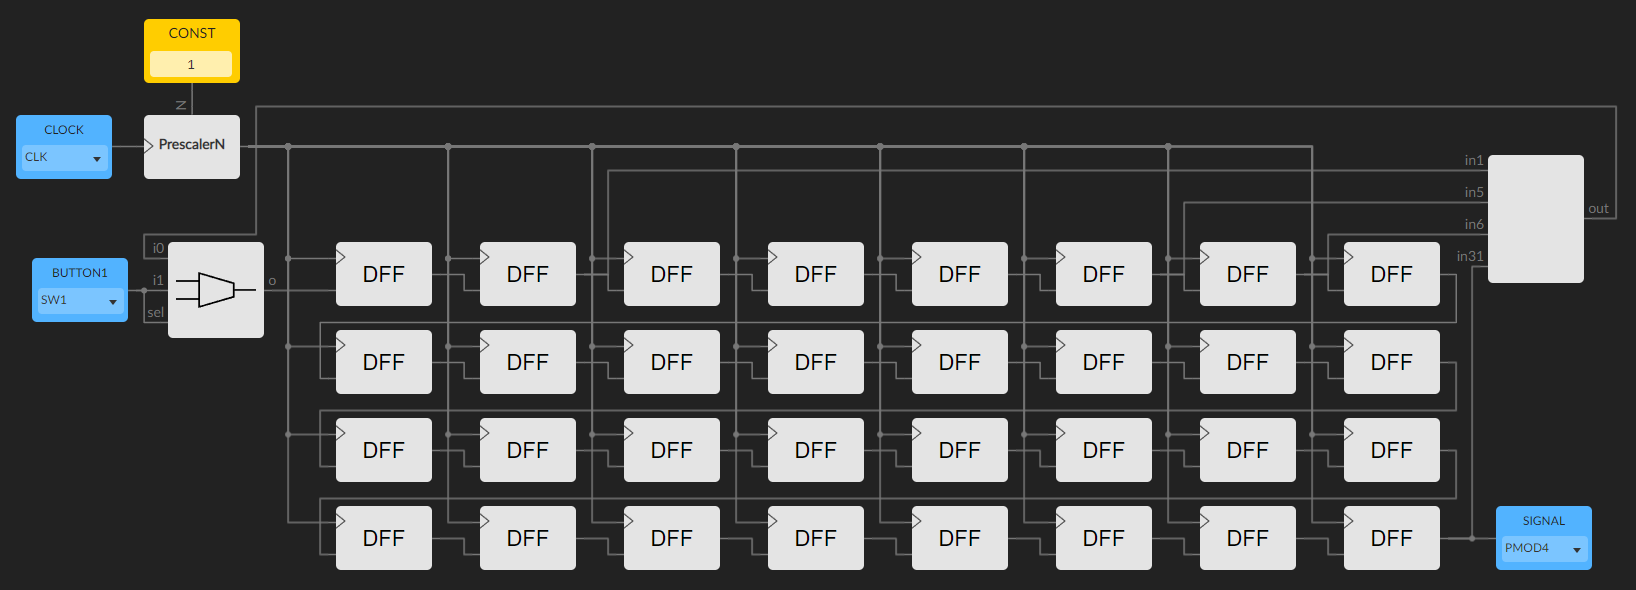
\includegraphics[scale=0.3]{./Images/03Research/ice.png}
	\caption{Kretsdiagram i Icestudio.}
	\label{fig:ICE}
\end{figure}

Med denne kretsen så ble frekvensspekteret fra 8KHz til 9KHz seende som vist i figur 

\begin{figure}[!hbt]
	\centering
	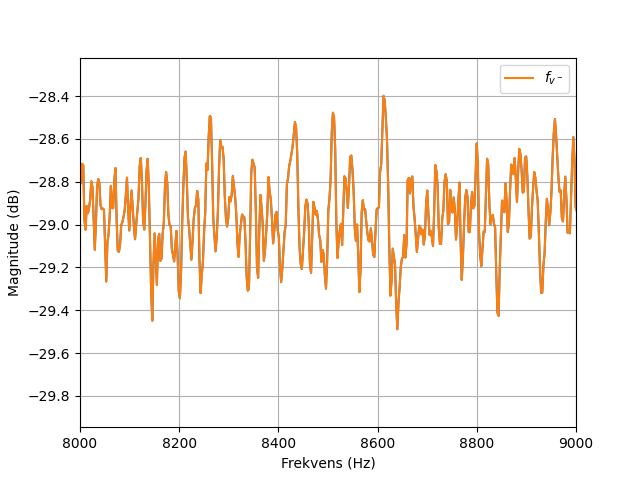
\includegraphics[scale=0.3]{./Images/03Research/spekter.png}
	\caption{Frekvensspekteret for intervallet [8KHz, 9KHz].}
	\label{fig:spekter}
\end{figure}

Ved måling av RMS eksponentiell gjennomsnitt så ble flatheten målt til 1.0962 dB i frekvensområdet [8KHz, 9KHz].
Ved lytting av signalet ble det observert hvit støy. Dette ble bekreftet ved sammenlikning med lydfilen i vevsiden \cite{wikipediacontributors_2022_white}.